% Created 2021-09-12 Sun 22:49
% Intended LaTeX compiler: xelatex
\documentclass[letterpaper]{article}
\usepackage{graphicx}
\usepackage{grffile}
\usepackage{longtable}
\usepackage{wrapfig}
\usepackage{rotating}
\usepackage[normalem]{ulem}
\usepackage{amsmath}
\usepackage{textcomp}
\usepackage{amssymb}
\usepackage{capt-of}
\usepackage{hyperref}
\usepackage[margin=1in]{geometry}
\usepackage{fontspec}
\usepackage{indentfirst}
\setmainfont[ItalicFont = LiberationSans-Italic, BoldFont = LiberationSans-Bold, BoldItalicFont = LiberationSans-BoldItalic]{LiberationSans}
\newfontfamily\NHLight[ItalicFont = LiberationSansNarrow-Italic, BoldFont       = LiberationSansNarrow-Bold, BoldItalicFont = LiberationSansNarrow-BoldItalic]{LiberationSansNarrow}
\newcommand\textrmlf[1]{{\NHLight#1}}
\newcommand\textitlf[1]{{\NHLight\itshape#1}}
\let\textbflf\textrm
\newcommand\textulf[1]{{\NHLight\bfseries#1}}
\newcommand\textuitlf[1]{{\NHLight\bfseries\itshape#1}}
\usepackage{fancyhdr}
\pagestyle{fancy}
\usepackage{titlesec}
\usepackage{titling}
\makeatletter
\lhead{\textbf{\@title}}
\makeatother
\rhead{\textrmlf{Compiled} \today}
\lfoot{\theauthor\ \textbullet \ \textbf{2021-2022}}
\cfoot{}
\rfoot{\textrmlf{Page} \thepage}
\titleformat{\section} {\Large} {\textrmlf{\thesection} {|}} {0.3em} {\textbf}
\titleformat{\subsection} {\large} {\textrmlf{\thesubsection} {|}} {0.2em} {\textbf}
\titleformat{\subsubsection} {\large} {\textrmlf{\thesubsubsection} {|}} {0.1em} {\textbf}
\setlength{\parskip}{0.45em}
\renewcommand\maketitle{}
\author{Houjun Liu}
\date{\today}
\title{The Electroscope}
\hypersetup{
 pdfauthor={Houjun Liu},
 pdftitle={The Electroscope},
 pdfkeywords={},
 pdfsubject={},
 pdfcreator={Emacs 28.0.50 (Org mode 9.4.4)}, 
 pdflang={English}}
\begin{document}

\maketitle


\section{The Electroscope}
\label{sec:org75f74a1}
\begin{figure}[htbp]
\centering
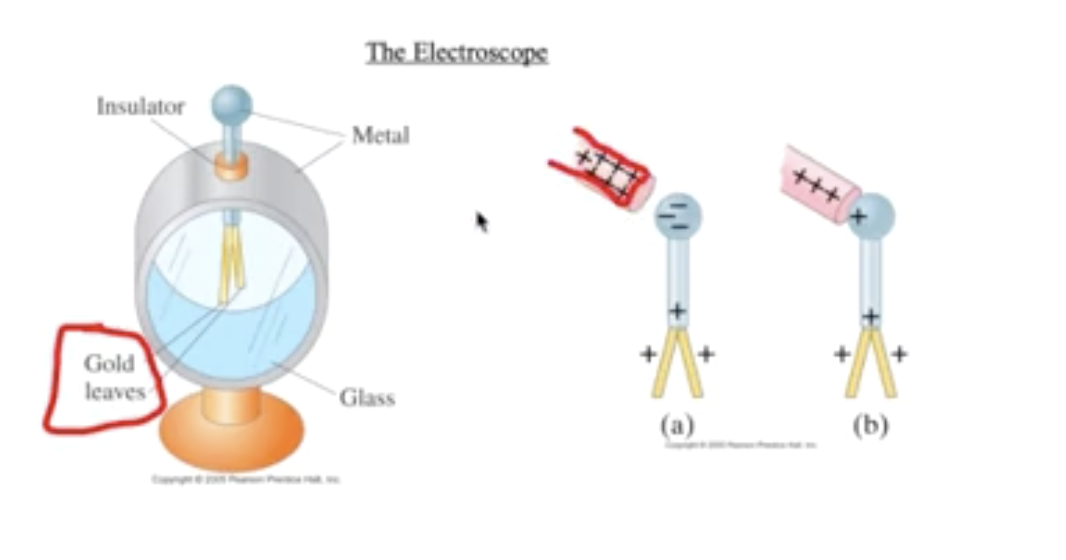
\includegraphics[width=.9\linewidth]{./2020PHYS201/Screen Shot 2020-08-24 at 7.31.10 PM.png}
\caption{Screen Shot 2020-08-24 at 7.31.10 PM.png}
\end{figure}

About how this works\ldots{}

\begin{enumerate}
\item Bring in some external charge near the electromitor (the ball-y part)
\item The rod becomes polarized, pushing the \(+\) protons down towards the
"gold leaves"

\begin{itemize}
\item If the rod is not close enough to cause electron flow but is close
enough to polarize\ldots{}

\begin{itemize}
\item Gold leaves temporarily push apart because positive repels
positives
\item When charged rod removed, leaves come back
\end{itemize}

\item If the rod is close enough to cause \(e^-\) to flow out of the
electromitor, making the whole rod more positive instead of a
temporary polarization\ldots{}

\begin{itemize}
\item Gold leaves permanently (until somebody/the air discharges it,
anyways) separated
\item When charged rod removed, leaves stay put
\end{itemize}
\end{itemize}
\end{enumerate}
\end{document}
